\chapter{Effectiveness of Existing Rule Sets}
This chapter considers different rule sets used for join enumeration in transformation based query optimization using Volcano/Cascades framework and analyse them for:  
\begin{itemize}
	\item Completeness : Ability to generate the space of all cross-product free join orders starting from an initial plan without cross products.
	\item Efficiency : Number of duplicates generated in the process of exploring the space. The lower the better.
\end{itemize}

We start with a basic rule set consisting of commutativity and associativity called rule set RS-B0. RS-B0 consists of redundant rules  and this redundancy is addressed in rule set RS-B1. Pellenkoft et al.\cite{pellenkoft1997complexity} showed that using RS-B1 leads to the generation of an exponential number of duplicates. They presented a new rule set RS-B2 which uses a new rule 'Exchange' in conjunction with RS-B0 and some added constraints to generate all alternate bushy join trees without generating duplicates. However we show that RS-B2 achieves this by generating trees outside of search space and a restriction to remain in search space leads to incompleteness.

\begin{defn} 
A Join Graph is a pair H = (V,E) where V is the set of base relations $R_{1},...,R_{n}$ and E is a set of edges. An edge between $R_{i}$ and $R_{j}$ indicates presence of join predicate between them. 
\end{defn}

\begin{defn} 
A Query Tree Q is a bushy plan showing the way the relations will be joined together.
\end{defn}

\section{Rule set RS-B0}
The simplest set of rules used (to generate the bushy space) are :

\begin{itemize}
	\item Left Associativity \\ $A \bowtie (B \bowtie C) \rightarrow (A \bowtie B) \bowtie C$
	\item Right Associativity \\ ($A \bowtie B) \bowtie C \rightarrow A \bowtie (B \bowtie C)$
	\item Commutativity \\ $A \bowtie B \rightarrow B \bowtie A$
\end{itemize}

\subsection{Efficiency}
The set is redundant because we can drop Left (or Right) Associativity and still generate the same space. This redundancy is addressed in rule set RS-B1. The number of duplicates is atleast as many as RS-B1.

\subsection{Completeness}
We show later in section \ref{rsb1complete} that a subset of these rules is sufficient to enumerate the entire space. 

\section{Rule set RS-B1}
Rule set RS-B1 consists of subset of rules of RS-B0 namely :
\begin{itemize}
	\item Left Associativity \\ $A \bowtie (B \bowtie C) \rightarrow (A \bowtie B) \bowtie C$
	\item Commutativity \\ $A \bowtie B \rightarrow B \bowtie A$
\end{itemize}

\subsection{Efficiency}
Pellenkoft et al. \cite{pellenkoft1997complexity} have shown that RS-B1 leads to exponential number of duplicates. The number of duplicates generated during the construction of MEMO-structure encoding all bushy trees for a clique join graph on n relations is $4^{n}-3^{n+1}+2^{n+2}-n-2$.

\subsection{Completeness}
\label{rsb1complete}

We show that this minimal set is sufficient to enumerate the cross product free space assuming the query is fully connected. \\

\textbf{Problem Description} : Given a connected join graph J and query tree Q, show that using RS-B1 we can reach any other valid query tree Q' from Q while remaining in cross-product free space. \\

We assume that Q itself does not have any cross products ie: Q belongs to search space. Given the input join graph $J$ is completely connected we can number the nodes $1,2...n$ such that $(..(R_{1}\bowtie R_{2})...)\bowtie R{n}$ is a valid left-deep join tree. To prove the problem statement, we prove a stronger claim : \\

\textbf{Claim 1} : Any query tree can be transformed into left-deep join tree and left-deep join tree can be transformed into any query tree in the search space. Hence to go from query tree $Q_{1}$ to $Q_{2}$, there exists atleast one route ie: $Q_{1}$ to left-deep tree to $Q_{2}$\\

Let us break the process on conversion from one tree to another into steps. In step 1 we move $R_{n}$ to the top so that it is last relation to be joined and then work on remaining set of relations numbered $1,2,..,n-1$. Generalized in step $i$, we move relation $R_{n-i+1}$ to the top and recurse on remaining relations 1 ... n-i. The decent stops when $i=n-1$. This brings us to Claim 2. \\

\textbf{Claim 2}: Having a query tree with relations $R_{1},R_{2},...R_{k}$, it is possible to build tree $[R_{1}R_{2}..R_{k-1}] \bowtie R_{k}$ where $[R_{1}R_{2}..R_{k-1}]$ represents a smaller join tree with relations $R_{1},R_{2},..R_{k-1}$ \\

Now the goal is given an query graph, move the highest numbered relation to the top so that its the last relation to be joined. Let k be the highest numbered relation and 1 .. k-1 are the other relations in the graph. View the tree as in Figure \ref{fig:rsb1-proof} where $C_{1}, C_{2}, ... C_{m}$ are equivalence classes consisting of some number of relations. We say the height of the tree is m+1. By induction on tree height, we show that $R_{k}$ can be brought to top while remaining in cross-product free space. \\

\begin{figure}[here]
\begin{center}
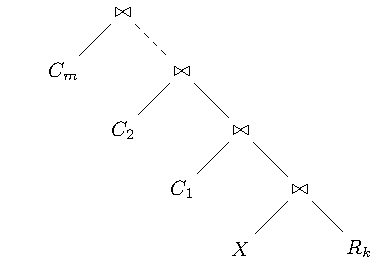
\includegraphics{Figures/rsb1-proof.pdf}
\end{center}
\caption{Reduced Query Tree}
\label{fig:rsb1-proof}
\end{figure}

Base Cases: When m = 0 , there is nothing to do, just repeat the procedure on X. When m = 1, X and $C_{1}$ should have a join predicate between them (because $R_{k}$ is the last relation to be join in left-deep tree). Applying left associativity we get required tree.\\

Induction on height m: Assume claim 2 holds for height $m <= j$. For height $m = j+1$, we know that since $R_{k}$ was the last relation to be joined in the left-deep tree, X can be joined with atleast one of the other C's say $C_{i}$. Pull $C_{i}$ down to X using a sequence of $C \rightarrow LA \rightarrow C$. Finally use Left Associativity to reduce height to j which is solvable. Hence Claim 2 proved, we can convert any tree into left-deep tree chosen earlier. \\

The last thing remaining to be shown is how we can go from left-deep tree to any other join tree. It is not difficult to see that this is equivalent to have the rules right associativity and commutativity and going from the join tree to left-deep tree. Right associativity can be done using a sequence of left associativity and commutativity : $RA \Rightarrow C \rightarrow C \rightarrow LA \rightarrow C$. We can use the same arguments as above to complete the proof.

\section{Rule set RS-B2}

Pellenkoft et al. \cite{pellenkoft1997complexity} presented a modified rule-set which generates the space of all bushy join trees with no duplicates. The rule set : 

\begin{itemize}
	\item $R_{1}$ : Commutativity \\ $A \bowtie_{0} B \rightarrow B \bowtie_{1} A$ \\
	Disable 	$R_{1}, R_{2}, R_{3}, R_{4}$ for application on new operator $\bowtie_{1}$
	\item $R_{2}$ : Left Associativity \\ $A \bowtie_{0} (B \bowtie_{1} C) \rightarrow (A \bowtie_{2} B) \bowtie_{3} C$ \\ 
	Disable 	$R_{2}, R_{3}, R_{4}$ for application  on new operator $\bowtie_{3}$	
	\item $R_{3}$ : Right Associativity \\ $(A \bowtie_{0} B) \bowtie_{1} C \rightarrow A \bowtie_{2} (B \bowtie_{3} C)$ \\
	Disable $R_{2}, R_{3}, R_{4}$ for application on new operator $\bowtie_{2}$	
	\item $R_{4}$ : Exchange \\ $(A \bowtie_{0} B) \bowtie_{1} (C \bowtie_{2} D) \rightarrow (A \bowtie_{3} C) \bowtie_{4} (B \bowtie_{5} D)$ \\
	Disable 	$R_{1}, R_{2}, R_{3}, R_{4}$ for application on new operator $\bowtie_{4}$
\end{itemize}

It is interesting to visualize the way exploration happens using RS-B2. Start at the topmost join operator, its left and right subtrees are completely explored. All the rules are applied at the top join operator and it gets locked. Now we explore all the newly generated join trees. In a way the locking happens one round from bottom to top, exchanges happen at the top(root) join operator and the root operator gets locked. Finally there is another round of locking happens this time from the top downwards. 

\subsection{Efficiency}
Pellenkoft et al. have showed that this scheme does not generate any duplicates and achieves the lower bound given by Ono and Lohman.


\subsection{Completeness}

\begin{figure}[ht]
\centering
\begin{subfigure}[b]{0.24\linewidth}
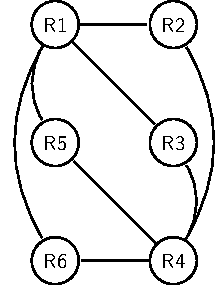
\includegraphics[width=2cm]{Figures/rsb2-predicates.pdf}
\caption{Join Graph J}
\label{fig:rsb2-counter}
\end{subfigure}
\begin{subfigure}[b]{0.35\linewidth}
	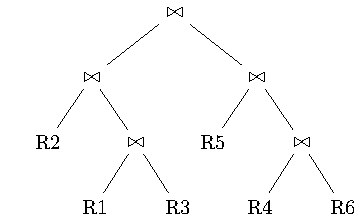
\includegraphics[width=3.5cm]{Figures/rsb2-counter.pdf}
\caption{Query Tree $Q$}
\label{fig:minipage1}
\end{subfigure}
\begin{subfigure}[b]{0.35\linewidth}
	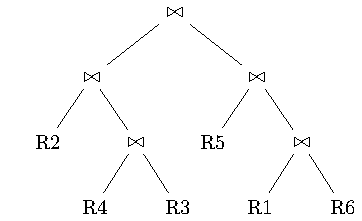
\includegraphics[width=3.5cm]{Figures/rsb2-counter2.pdf}
\caption{Query Tree $Q_{2}$}
\label{fig:minipage2}
\end{subfigure}
\end{figure}
RS-B2 cannot generate the space of all bushy trees without cross products. Given a set of relations to be joined with join graph $J$ (Figure \ref{fig:rsb2-counter}) and initial query tree $Q$ (Figure \ref{fig:minipage1}), observe that swapping R1 and R4 will lead to a valid query tree $Q_2$ (Figure \ref{fig:minipage2}) which does not have any cross product. Hence $Q_2$ belongs to search space. However going from $Q$ to $Q_2$ would require formation of sub-tree $R_2$,$R_3$ which will lead to cross product.